% !TEX root = ../proposal.tex

 \renewcommand{\arraystretch}{0.75}
\begin{table}[t]
\begin{center}
{  \fontsize{9}{11pt}\selectfont
\begin{tabular}{|l|p{7.9cm}|p{1.35cm}|p{0.8cm}|p{0.9cm}|p{0.9cm}|}
\hline
\highlightCell WP & \highlightCell Work package title &  \highlightCell Leader (no) & \highlightCell PMs & \highlightCell Start month & \highlightCell End month
\\ \hline\hline

\WPSpecification &
\textbf{Req., System \& Component Spec. and Arch.}\newline
 {\scriptsize
 Task~\WPSpecificationNo.1: End-user needs and requirements analysis
 \newline
 Task~\WPSpecificationNo.2: Application analysis and requirement specification
 \newline
 Task~\WPSpecificationNo.3: Definition and specification of system architecture
 \newline
 Task~\WPSpecificationNo.4: System hardware and software components specification
 }
 & \CLUJ\newline(\CLUJNo)  &
\WPSpecificationSUM
& M1 & M28
\\ \hline

%-------------------------------

\WPVehicle &
{\bf \WPVehicleTitle}\newline
 {\scriptsize
 Task~\WPVehicleNo.1: Vehicle platform setup
 \newline
 Task~\WPVehicleNo.2: Drive by wire functionality
 \newline
 Task~\WPVehicleNo.3: Low-level data acq., proc. \& comm. framework
 \newline
 Task~\WPVehicleNo.4: High level system debugging \& maintenance framework
 \newline
 Task~\WPVehicleNo.5: Calibration \& data integrity validation of the sensor system
 \newline
 Task~\WPVehicleNo.6: Reference sensor integration
 \newline
 Task~\WPVehicleNo.7: Vehicle maintenance and update
 }
 & \VW\newline(\VWNo)  &
\WPVehicleSUM
& M1 & M28
\\ \hline

%-------------------------------

\WPCloud &
{\bf \WPCloudTitle}\newline
 {\scriptsize
 Task~\WPCloudNo.1: Setup of project-wide development infrastructure
 \newline
 Task~\WPCloudNo.2: Setup of hardware stack
 \newline
 Task~\WPCloudNo.3: Design and impl. of the devel. and deployment tool chain
 \newline
 Task~\WPCloudNo.4: Setup and implementation of a communication framework
\newline
 Task~\WPCloudNo.5: Setup and implementation of the bulk data storage service
 \newline
% Task~\WPCloudNo.6: Setup and impl. of a server-side monitoring service
 }
 & \IBM\newline(\IBMNo)  &
\WPCloudSUM
& M1 & M32
\\ \hline

%-------------------------------

\WPPerception &
{\bf \WPPerceptionTitle}\newline
 {\scriptsize
 Task~\WPPerceptionNo.1: Specification and design of on-board sensing
% \newline
% Task~\WPPerceptionNo.2: System-wide data acquisition
 \newline
 Task~\WPPerceptionNo.2: Spatio-temporal and appearance based low level rep.
 \newline
 Task~\WPPerceptionNo.3: Perception adaptation to adverse visibility conditions
\newline
 Task~\WPPerceptionNo.4: Road infrastructure perception
 \newline
 Task~\WPPerceptionNo.5: Real-time 3D terrain perception
 \newline
 Task~\WPPerceptionNo.6: Road users perception \& signaling detection
 \newline
 Task~\WPPerceptionNo.7: Sensor fusion based perception refinement
 }
 & \CLUJ\newline(\CLUJNo)  &
\WPPerceptionSUM
& M1 & M42
\\ \hline

%-------------------------------

\WPMapping &
{\bf \WPMappingTitle}\newline
 {\scriptsize
 Task~\WPMappingNo.1: Mapping frontend
 \newline
 Task~\WPMappingNo.2: Internal map representation
 \newline
 Task~\WPMappingNo.3: Internal map storage
 \newline
 Task~\WPMappingNo.4: Highly accurate metric localization
\newline
 Task~\WPMappingNo.5: Classification and aggregation of semantic data
 \newline
 Task~\WPMappingNo.6: Map management and summarization
 \newline
 %Task~\WPMappingNo.7: Evaluation of the lifelong loc. \& mapping performance
 }
 & \ETHZ\newline(\ETHZNo)  &
\WPMappingSUM
& M1 & M42
\\ \hline

%-------------------------------

\WPSceneUnderstanding &
{\bf \WPSceneUnderstandingTitle}\newline
 {\scriptsize
 Task~\WPSceneUnderstandingNo.1: Long-term semantic scene understanding
 \newline
 Task~\WPSceneUnderstandingNo.2: Scenario based scene understanding
 \newline
 Task~\WPSceneUnderstandingNo.3: Scene prediction
 \newline
 Task~\WPSceneUnderstandingNo.4: Self-assessment
 }
 & \PRAGUE\newline(\PRAGUENo)  &
\WPSceneUnderstandingSUM
& M3 & M44
\\ \hline

%-------------------------------

\WPNavigation &
{\bf \WPNavigationTitle}\newline
 {\scriptsize
 Task~\WPNavigationNo.1: Route planning
 \newline
 Task~\WPNavigationNo.2: Tactical planning
 \newline
 Task~\WPNavigationNo.3: Trajectory planning
 \newline
 Task~\WPNavigationNo.4: Trajectory control
 \newline
 Task~\WPNavigationNo.5: Mission Executive
 }
 & \VW\newline(\VWNo)  &
\WPNavigationSUM
& M3 & M46
\\ \hline

%-------------------------------

\WPIntegration &
{\bf \WPIntegrationTitle}\newline
 {\scriptsize
 Task~\WPIntegrationNo.1: Integration Plan
 \newline
 Task~\WPIntegrationNo.2: System-wide data acquisition
 \newline
 Task~\WPIntegrationNo.3: Integration and test tools and processes
 \newline
 Task~\WPIntegrationNo.4: System integration
 \newline
 Task~\WPIntegrationNo.5: System evaluation and validation
  }
 & \VW\newline(\VWNo)  &
\WPIntegrationSUM
& M2 & M48
\\ \hline

%-------------------------------

\WPInnovation &
{\bf \WPInnovationTitle}\newline
 {\scriptsize
 Task~\WPInnovationNo.1: Management of knowledge
 \newline
 Task~\WPInnovationNo.2: Dissemination
 \newline
 Task~\WPInnovationNo.3: Exploitation
  }
 & \IBM\newline(\IBMNo)  &
\WPInnovationSUM
& M1 & M48
\\ \hline

%-------------------------------

\WPManagement &
{\bf \WPManagementTitle}\newline
 {\scriptsize
 Task~\WPManagementNo.1: Project management
 \newline
 Task~\WPManagementNo.2: Project status monitoring
  }
 &  \COORD \newline (\COORDNo) &
\WPManagementSUM
 & M1 & M48
\\ \hline\hline
-- & TOTAL &   -- &
\PMSUM
& --  & --
\\ \hline
\end{tabular}
}
\caption{Work package and task overview. }
   \label{tab:wpoverview}
\end{center}
\end{table}

Table~\ref{tab:wpoverview} on Page~\pageref{tab:wpoverview} provides an {\bf overview over the work packages} by listing the tasks addressed in
the individual work packages.

 \renewcommand{\arraystretch}{1.0}

%------------------------------------------------------------------

\begin{table}[t]
  \centering
  {  \fontsize{9}{11pt}\selectfont
\begin{tabular}{|l|p{7.6cm}|p{0.9cm}|p{1.6cm}|p{0.9cm}|p{0.7cm}|p{1.5cm}|}
\hline
\highlightCell No. & \highlightCell Deliverable name & \highlightCell WP &  \highlightCell Resp. partner & \highlightCell Type & \highlightCell Diss. level & \highlightCell Del. Date
\\ \hline\hline
D1.1 & Initial version of requirements definition, system architecture and component specification & WP1 & \CLUJ & R & PU & M4 \\\hline
D1.2 & Final version of requirements definition, system architecture and component specification & WP1 & \CLUJ & R & PU & M28 \\\hline\hline

%----------------------------------

D2.1 & First vehicle platform available & WP2 & \VW & R & PU & M8 \\\hline
D2.2 & First vehicle platform fully operational & WP2 & \VW & R & PU & M12 \\\hline
D2.3 & Second vehicle platform available & WP2 & \VW & R & PU & M24 \\\hline
D2.4 & Second vehicle platform fully functional & WP2 & \VW & R & PU & M28 \\\hline\hline

%----------------------------------

D3.1 & Development infrastructure & WP3 & \IBM & R & PU & M1 \\\hline
D3.2 & Hardware stack  & WP3 & \IBM & R & PU & M4(i), M28 \\\hline
D3.3 & Development and deployment tool chain & WP3 & \IBM & R & PU & M8 \\\hline
D3.4 & Communication framework  & WP3 & \IBM & R & PU & M12 \\\hline
D3.5 & Bulk data storage service  & WP3 & \IBM & R & PU & M16 \\\hline\hline
%----------------------------------

D4.1 & Specification and design of on-board sensing & WP4 & \CLUJ & R & PU & M8(i), M28 \\\hline
D4.2 & Low-level perception functions & WP4 & \CLUJ & R & PU & M18(i), M32 \\\hline
D4.3 & Higher-level perception functions  & WP4 & \CLUJ, \PRAGUE, \VW & R & PU & M18(i), M42 \\\hline\hline

%----------------------------------

D5.1 & Specification of the map frontend and storage concept & WP5 & \ETHZ & R & PU & M4 \\\hline
D5.2 & First development and integration cycle of lifelong mapping & WP5 & \ETHZ & R & PU & M18 \\\hline
D5.3 & Second development and integration cycle of lifelong mapping & WP5 & \IBM & R & PU & M42 \\\hline\hline
%D5.5 & Evaluation of the lifelong mapping performance & WP5 & \ETHZ & R & PU & M48 \\\hline\hline

%----------------------------------

D6.1 & Software specification and architecture for scene understanding & WP6 & \PRAGUE & R & PU & M6 \\\hline
D6.2 & First development and integration cycle of scene understanding  & WP6 & \PRAGUE & R & PU & M20 \\\hline
D6.3 & Second development and integration cycle of scene understanding  & WP6 & \PRAGUE & R & PU & M44 \\\hline\hline

%----------------------------------

D7.1 & Software specification and architecture for the decision making and navigation & WP7 & \VW & R & PU & M6 \\\hline
D7.2 & First development and integration cycle of decision making and navigation & WP7 & \VW & R & PU & M22 \\\hline
D7.3 & Second development and integration cycle of decision making and navigation & WP7 & \VW & R & PU & M46 \\\hline\hline

%----------------------------------

D8.1 & Integration plan for first development cycle & WP8 & \VW & R & INT & M12 \\\hline
D8.2 & Initial component and system data sets & WP8 & \VW & R & INT & M14 \\\hline
D8.3 & Integration and test tools and processes & WP8 & \VW & R & PU & M16 \\\hline
D8.4 & Evaluation report on integration process and results of first development cycle & WP8 & \VW & R & PU & M24 \\\hline
D8.5 & Integration plan for second development cycle & WP8 & \VW & R & INT & M30 \\\hline
D8.6 & Evaluation report on integration process and results of second development cycle & WP8 & \VW & R & PU & M48 \\\hline\hline

%----------------------------------

D9.1 & Project Web-page  & WP9 & \ETHZ  & DEC & PU & M2 \\\hline
D9.2 & Data management plan & WP9 & \ETHZ & R & PU & M4 \\\hline
D9.3 & Brochure, newsletter & WP9 & \PRAGUE & DEC & PU & M16 \\\hline
D9.4 & Press video & WP9 &  \IBM &  DEC & PU & M27 \\\hline
D9.5 & Exploitation plan & WP9 & \IBM & R & INT & M18(i), M40 \\\hline
D9.6 & Dissemination report & WP9 & \PRAGUE  & R & PU & M21(i), M45 \\\hline
D9.7 & Final demonstration & WP9 & \VW & DEC & PU & M24(i), M48 \\\hline


\end{tabular}
[R] Report, [DEC] press \& media action, [PU] Public, [INT] Internal, (i) intermediate version
}
  \caption{List of Deliverables}
  \label{tab:deliverables}
\end{table}


%---------------------------------------------------------------


\begin{figure}
\begin{center}
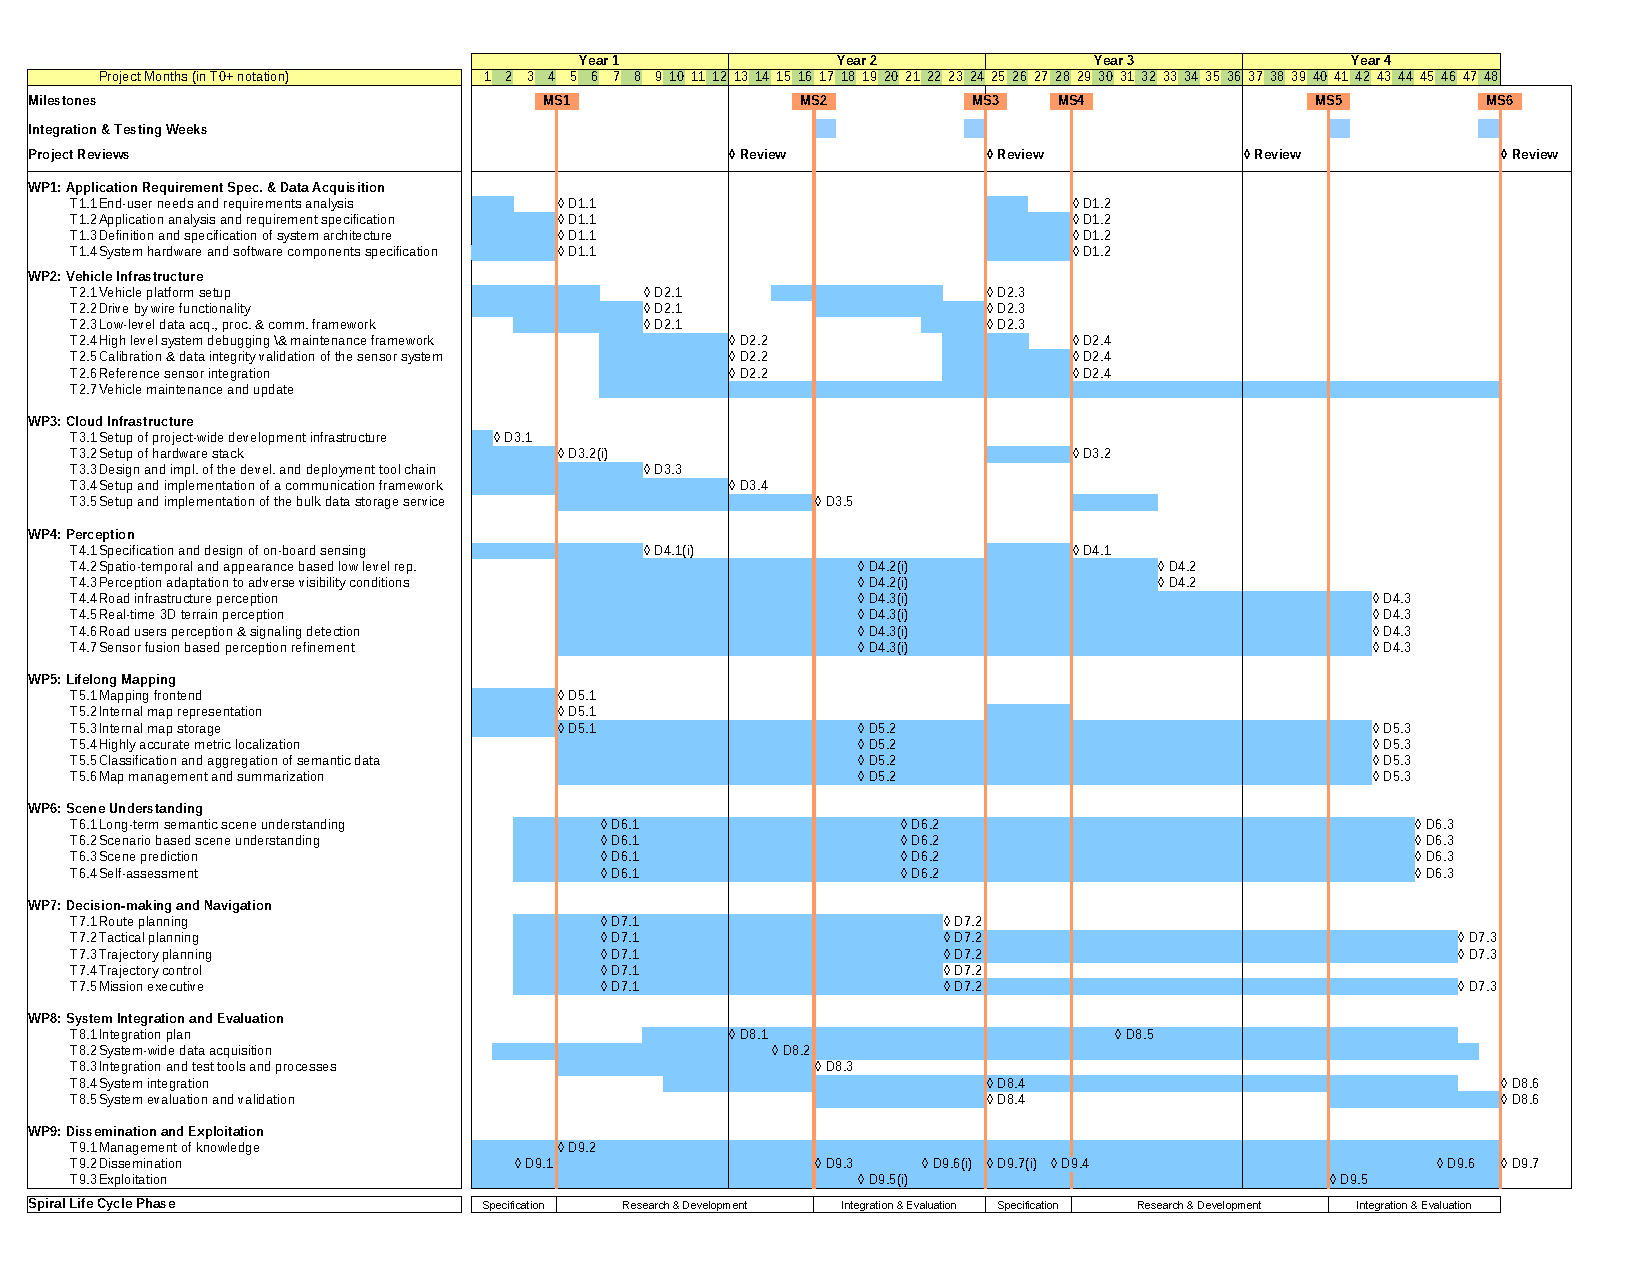
\includegraphics[angle=90,height=0.95\textheight]{pics/gantt}
\caption{Gantt chart over the whole period of the project illustrating the tasks in the work packages as well as  the Milestones and Deliverables.}
\label{fig:gantt}
\end{center}
\end{figure}


